\documentclass[12pt]{article}
\usepackage[utf8]{inputenc}
\usepackage{graphicx}
\usepackage{hyperref}
\usepackage{xurl}
\usepackage[table]{xcolor}
\usepackage[dvipsnames]{xcolor}
% Place Page X of Y on the right-hand
% side of the footer
\usepackage{geometry}
 \geometry{
 a4paper,
 total={170mm,257mm},
 left=25mm,
 right=25mm,
 top=25mm,
 }

\begin{document}
\begin{titlepage}
	\centering
	\includegraphics[width=0.3\textwidth]{indir.png}\par\vspace{1cm}
	{\scshape\large Università degli Studi di Padova \par}
	\vspace{1cm}
	{\scshape\normalsize Web Application Project\par}
	\vspace{1cm}
	    {\Large\bfseries FIRST REPORT
     \par}
     \vspace{1cm}
	{\Large\bfseries  WAVE PROJECT WEB APPLICATION
\par}
	\vspace{1cm}
	{\large {Written By}\par}
	\vspace{1cm}
	{\large\itshape Meltem Yanoğlu\par}
	{\large\itshape Umut Berk Çakmakçı\par}
	\vfill
	Supervisor\par
	Prof. Nicolo Ferro

	\vfill

{\large \today\par}
\end{titlepage}
\small\tableofcontents
\newpage

\section{Objectives}
\bigskip
\paragraph{} 


\section{Main Functionalities}
\bigskip
\paragraph{} 
\subsection{Main Area}
\subsection{Admin Area}
\subsection{Customer Area}


\section{Data Logic Layer}
\bigskip
\paragraph{} 
\subsection{ER (Entity-Relationship) Diagram}

\newpage
\section{Presentation Logic Layer}
\bigskip
\paragraph{} 
Our website will be divided into some sections. You can find them below. 
\begin{itemize}

    \item Home: our home page contains Sign Up, Sign In button for users who want to sign in or sign up into the website, About Us and Contact Us sections.
    
%    \item Sign up: allows users to register into the website.
%    \item Sign in: allows users to login to the website. 
%    \item Forget password: allows users who already registered to the website reset their password.  
    
    \item Admin: allows admins control the website, customers and products. 
    \item Customer details: allows admins see the customers's detailed profiles, edit information's, delete and add new customers.  
    
%    \item Add customer: allows admins add a new customer. 
%    \item Edit customer: allows admins edit an existing customer information.
    
    \item Product details: allows admins to see the products' details, edit information's, delete and add new products. 
    
%    \item Add product: allows admins add a new product. 
%    \item Edit product: allows admins edit an existing product’s details. 
    
    \item Cart: allows customers to see and manage the products they choose. 	
    \item Contact us: allows customers to send a message to website admins. 
\end{itemize}

\newpage
\subsection{Home Page}
\bigskip
\paragraph{}
The Home page will show the clothes’ categories like winter/summer,  male/\newline female/kids, skirt/short/jeans, etc. Once the customer clicks one of the categories in the home page, all the clothes belong to that category will be displayed. 
\paragraph{}
The Home page contains Sign Up/In button, Sign In button for customers who already registered the system and Sign Up button for customers who will register the system for the first time. Pressing Sign Up/In button will direct customers to Sign In page. If the customer has no account, they should click Create Account button and the system will direct customers to the Sign Up page.
\paragraph{}
The home page also contains About Us and Contact Us buttons. In About Us page, there will be general information related with the company, headquarter’s address, tax code and social media links. Contact Us page will be used for our customers to get in touch with officials. Our Centers page will show our stores’ addresses and locations all over the globe. And lastly, the shopping cart symbol will direct customers to the products they add into their cart.

\bigskip
\bigskip
\bigskip
\begin{figure}[h]
\centerline{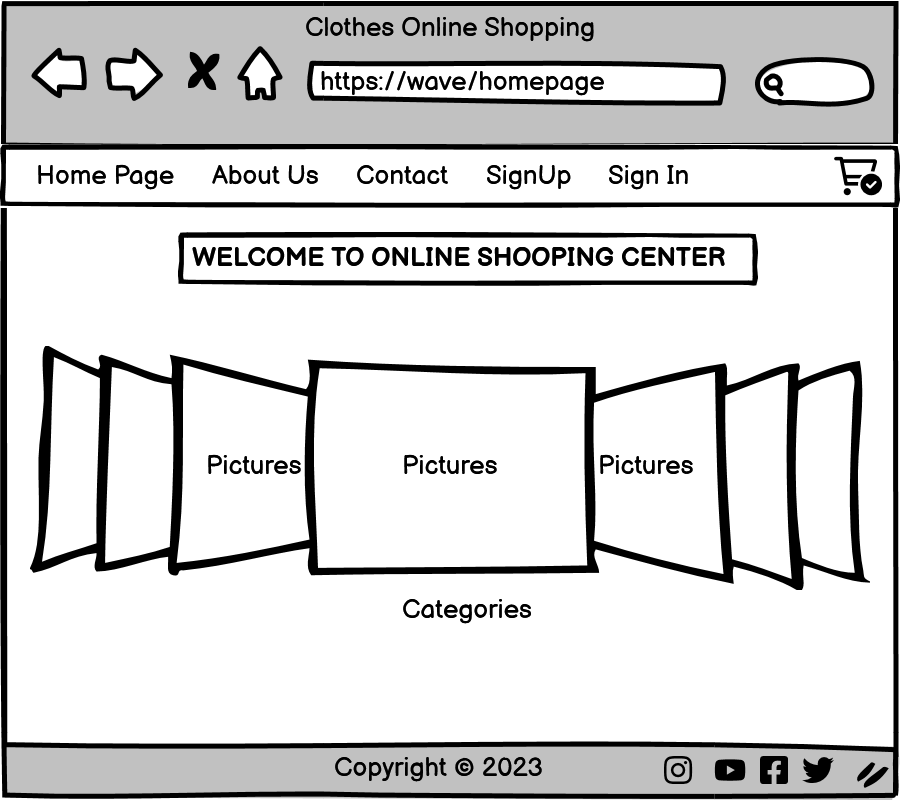
\includegraphics[scale=1]{images/Home.png}}
\caption{Home Page}
\label{fig}
\end{figure}

\newpage
\subsection{Sign Up Page}
\bigskip
\paragraph{}
In Sign Up page, customers can register into the website by filling the required fields like name, e-mail, password, phone and address. After filling these fields, the customer can click Register button and the customer will be registered into the system. Customers who already has an account can click the Already Register button and go to the Sign In page. 

\bigskip
\bigskip
\bigskip
\begin{figure}[h]
\centerline{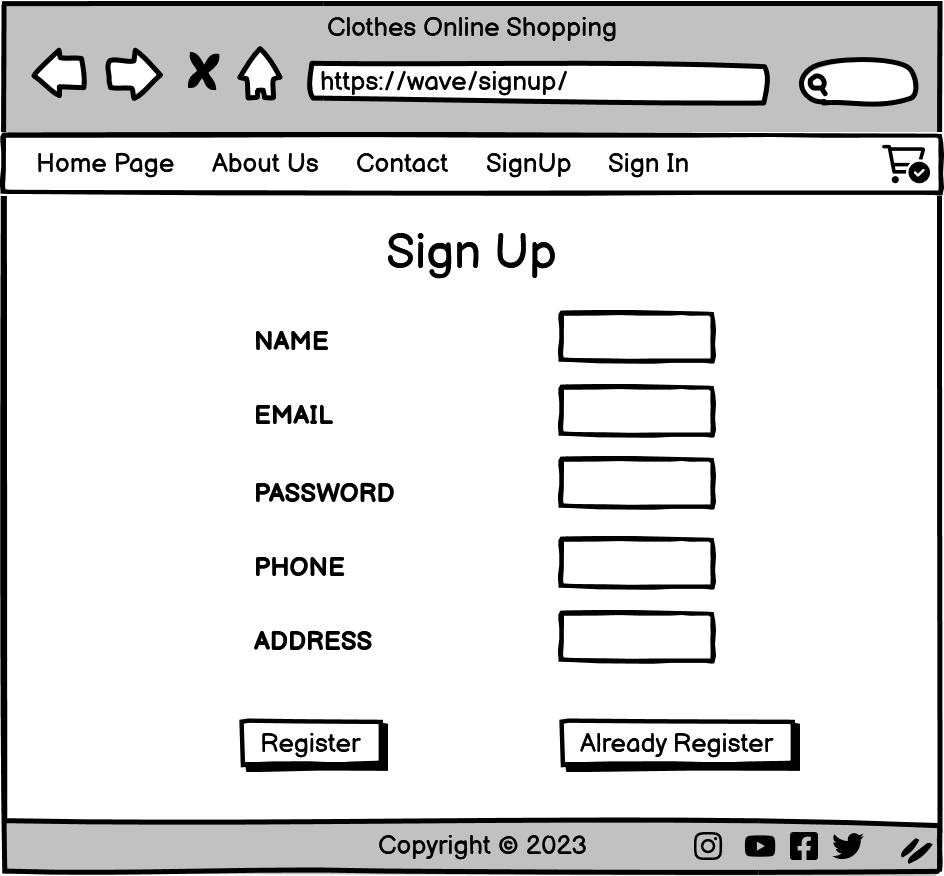
\includegraphics[scale=1.]{images/Sign Up.png}}
\caption{Sign Up Page}
\label{fig}
\end{figure}

\newpage
\subsection{Sign In Page}
\bigskip
\paragraph{}
In Sign In page, customers who has an account, can sign in the website by filling the e-mail and password. If the customer forgot his/her password, can click the Forget Password button and go to the password reset page. Customer who does not have an account can click the Create Account button and directed to the Sign Up page. 

\bigskip
\bigskip
\bigskip
\begin{figure}[h]
\centerline{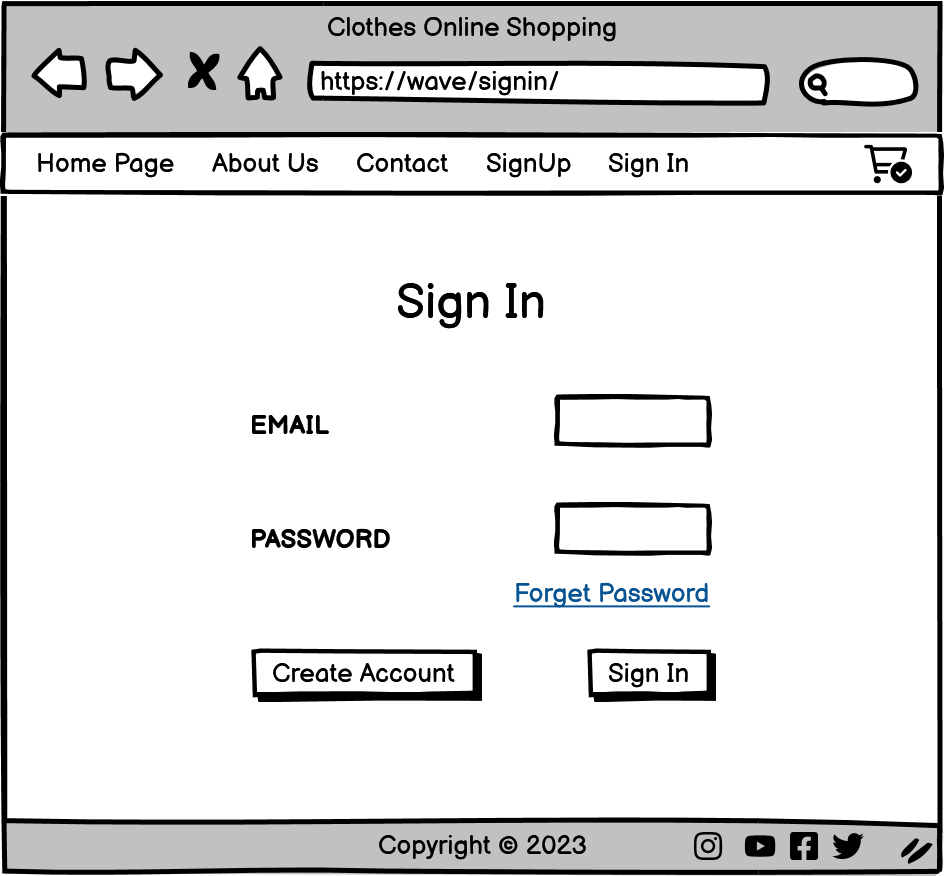
\includegraphics[scale=1.]{images/Sign In.png}}
\caption{Sign In Page}
\label{fig}
\end{figure}

\newpage
\subsection{Forget Password Page}
\bigskip
\paragraph{}
In Forget Password page, customers who has an account, can reset their password if they forgot or want to change it. When the customer click the button Forget Password, the system sends an automatic e-mail with a link which directs the customer to the Reset Password page. In this page, customers can type their new password twice and click the Reset button and the system automatically update the password related with that e-mail address in the database. 
\bigskip
\bigskip
\bigskip
\begin{figure}[h]
\centerline{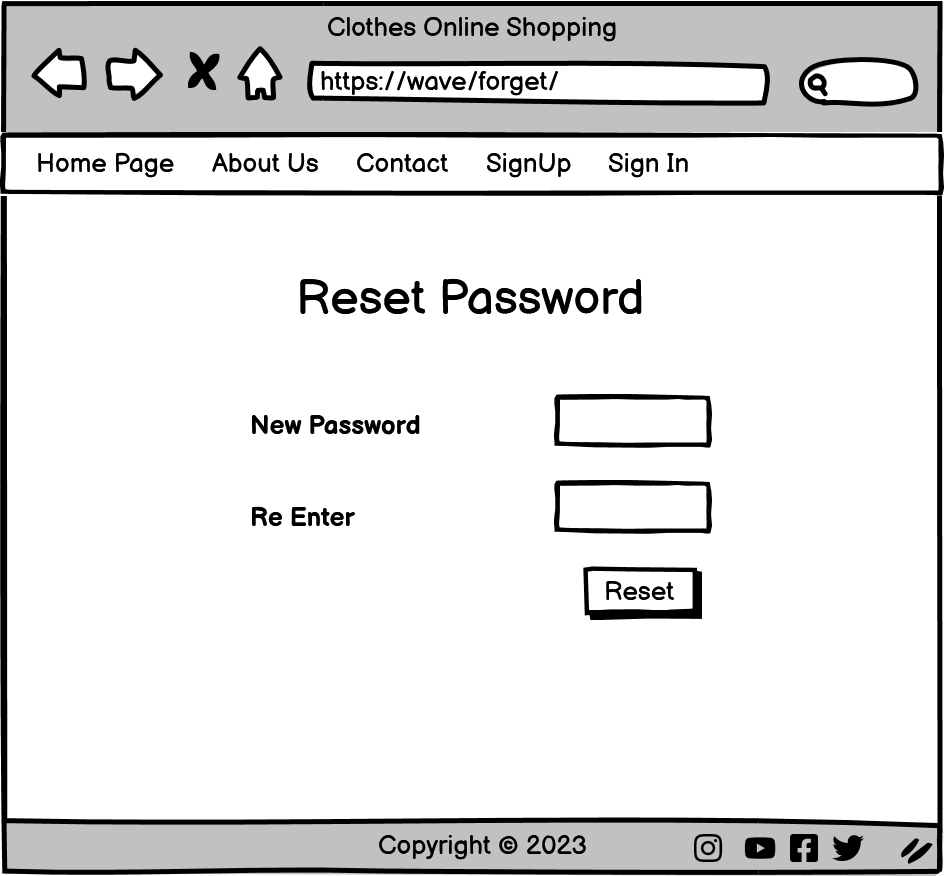
\includegraphics[scale=1.]{images/Forget Password.png}}
\caption{Forget Password Page}
\label{fig}
\end{figure}

\newpage
\subsection{About Us Page}
\bigskip
\paragraph{}
In About Us page, the customer can get information about the company and it's products. Also customers can find information about the addresses of the physical stores of the company and all the branches and their locations. This page has a map that shows the locations of the centers and branches of the shops.
\bigskip
\bigskip
\bigskip
\begin{figure}[h]
\centerline{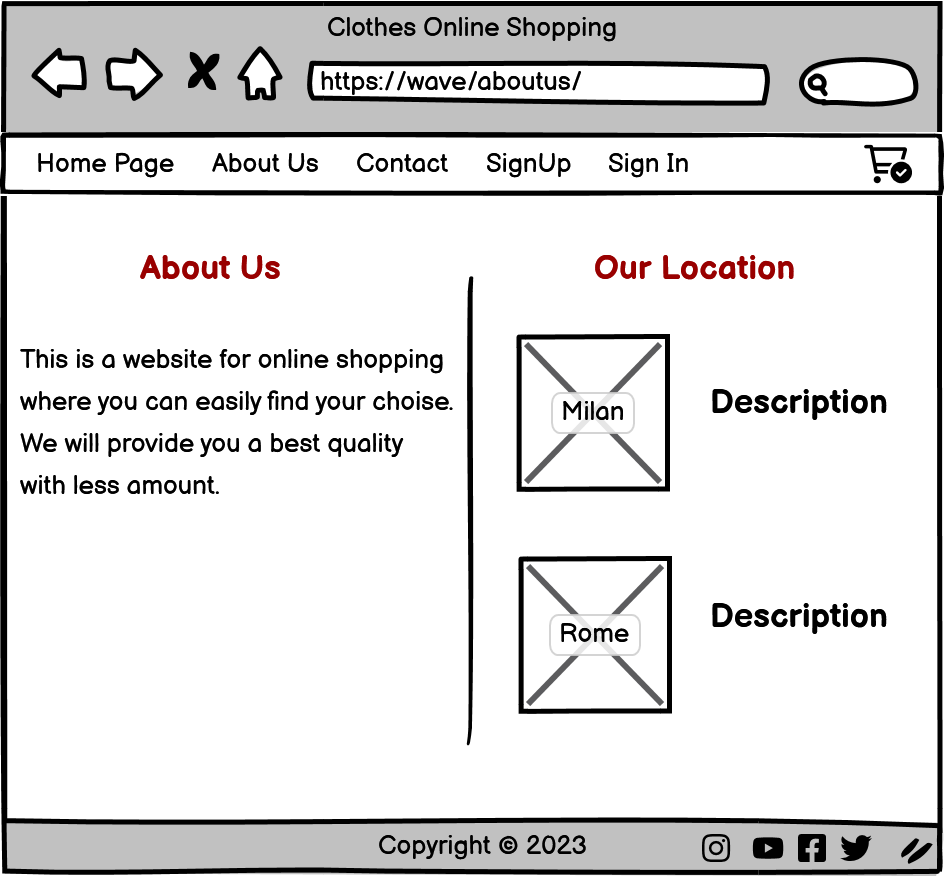
\includegraphics[scale=1.]{images/About Us.png}}
\caption{About Us Page}
\label{fig}
\end{figure}


\newpage
\subsection{Contact Us Page}
\bigskip
\paragraph{}
In Contact Us page, customers who has a compliment or suggestion or such that, can get in touch with the admins/officials of the company tell what they want to tell. Once the customer fill the form with necessary fields, e-mail, name and Type Message fields, they can click the Send Message button and send their message. An automatic notification e-mail related with the message's delivery will be sent to the customer's e-mail address. 
\bigskip
\bigskip
\bigskip
\begin{figure}[h]
\centerline{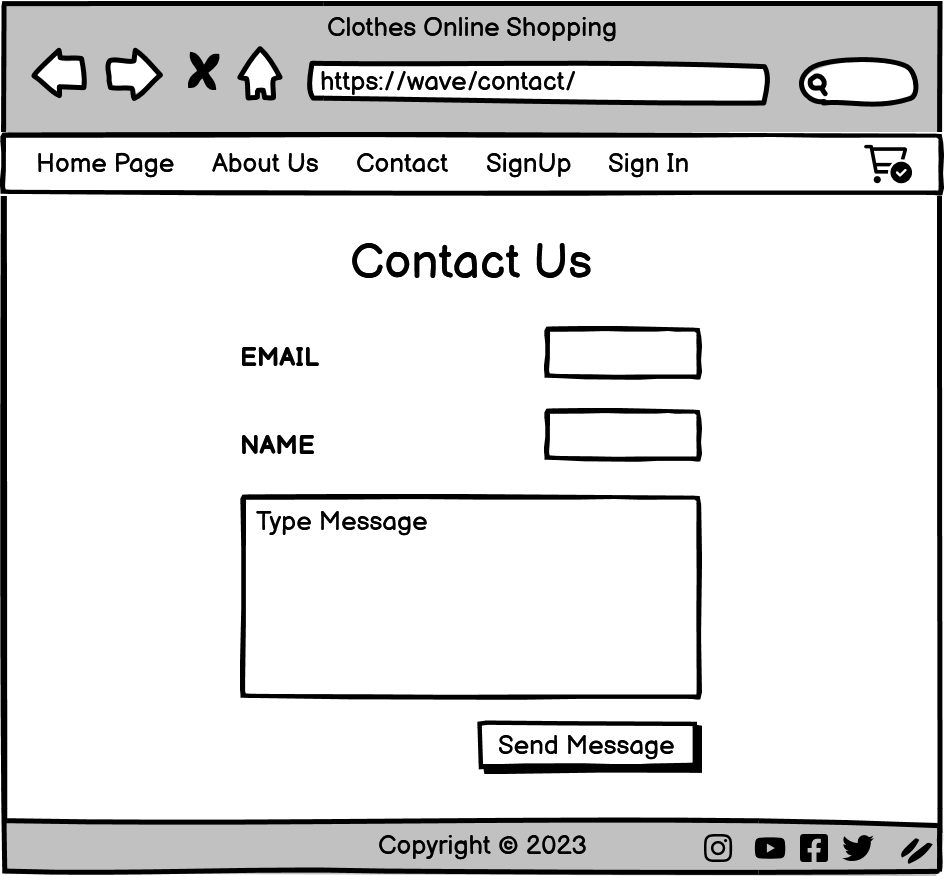
\includegraphics[scale=1.]{images/Contact Us.png}}
\caption{Contact Us Page}
\label{fig}
\end{figure}

\newpage
\subsection{Admin Page}
\bigskip
\paragraph{}
The Admin Page consists of 3 main section; Total Products, Purchased Products, and Registered Customers. With these 3 sections, the website admins can see and control the products and customers. Admins can see the total products they have, how many products they sell and total registered customers with all the details. They also can add new product/customer and edit the existing ones. 

\bigskip
\bigskip
\bigskip
\begin{figure}[h]
\centerline{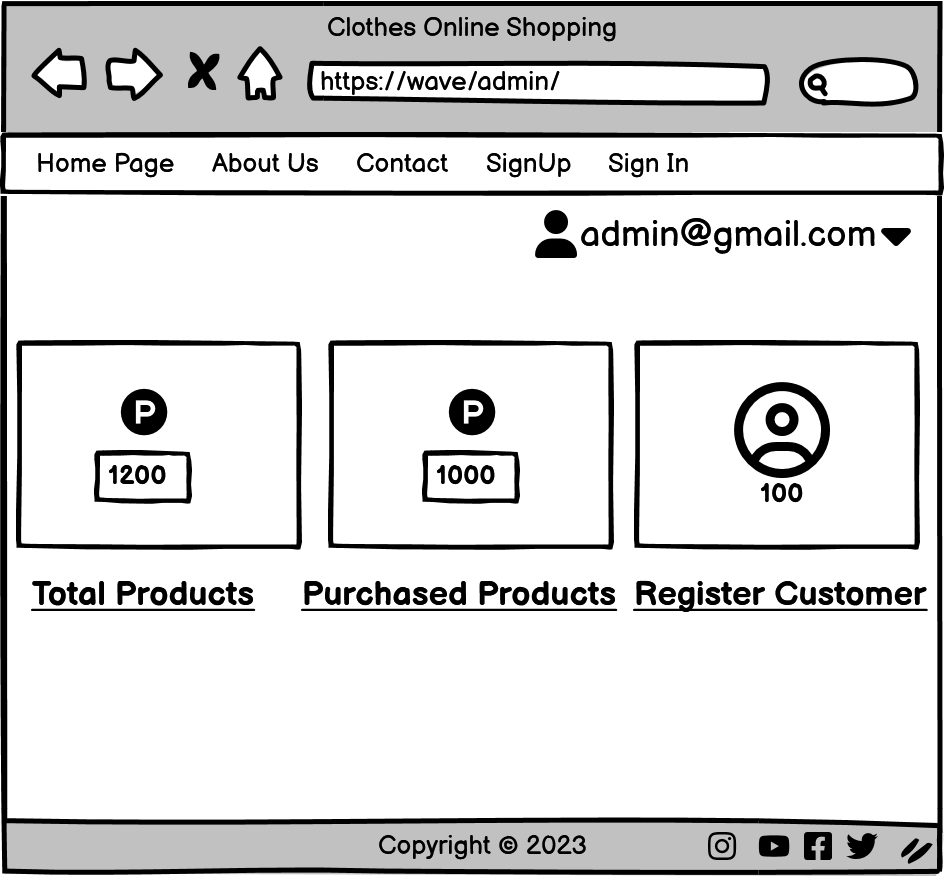
\includegraphics[scale=1.]{images/Admin.png}}
\caption{Admin Page}
\label{fig}
\end{figure}

\newpage
\subsection{Customer Details Page}
\bigskip
\paragraph{}
In Customer Details page, there is a table that contains all the registered customers' detailed information like phone numbers and addresses. Website admins can see and modify the customers information, add new customer or delete an existing one. Select one customer from the table and then click Edit button, admins can edit that customer's information. Or by clicking the Delete button, admin can delete one existing customer from website and also from the database. On the other hand, if admin want to add new customer to the system, he/she click the Add button and add customer. 
\bigskip
\bigskip
\bigskip
\begin{figure}[h]
\centerline{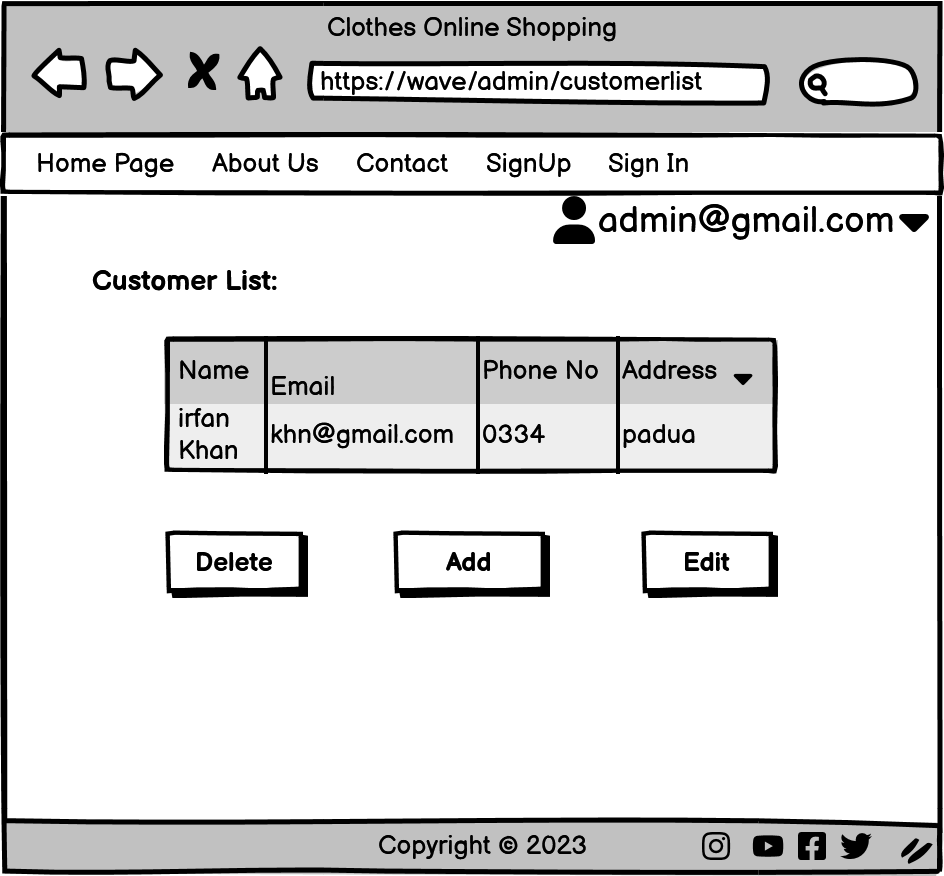
\includegraphics[scale=1.]{images/Customer Details.png}}
\caption{Customer Details Page}
\label{fig}
\end{figure}

\newpage
\subsection{Add Customer Page}
\bigskip
\paragraph{}
In Add Customer page, admin will fill manually the required fields; name, e-mail, password, phone number and address, and then, click the Add button at the end of the page. By clicking the Add button, new customer is created and added to the system and database. A notification e-mail will be sent to the customer's e-mail address. 
\bigskip
\bigskip
\bigskip
\begin{figure}[h]
\centerline{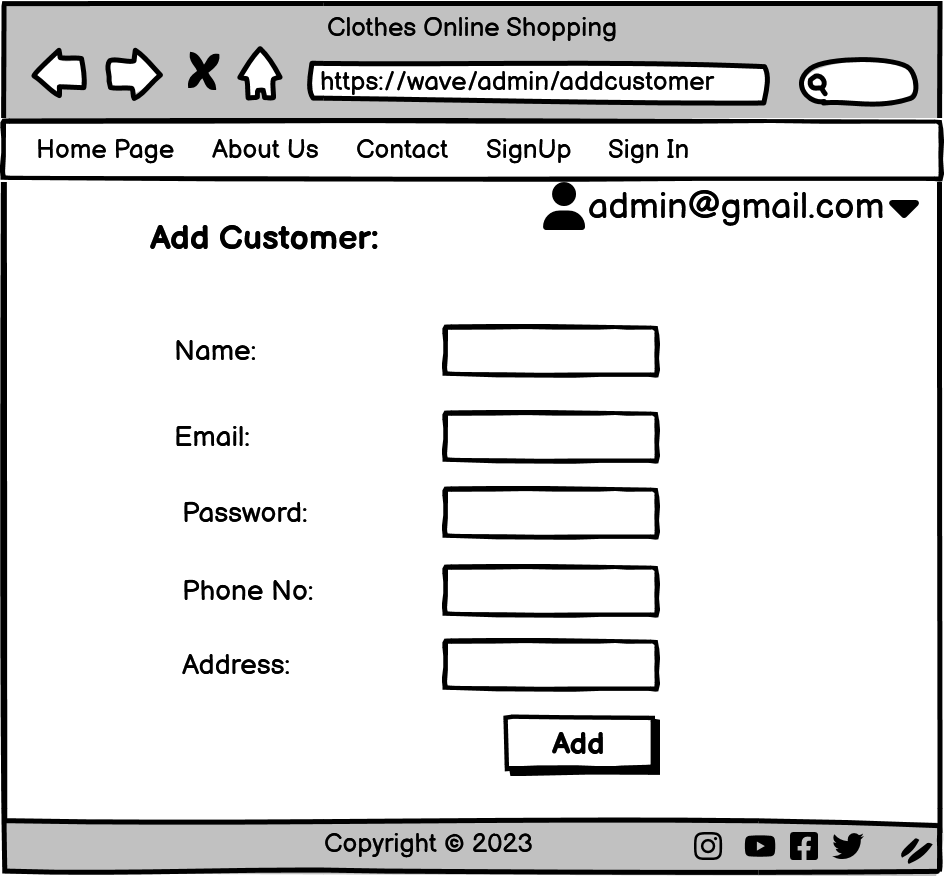
\includegraphics[scale=1.]{images/Add Customer.png}}
\caption{Add Customer Page}
\label{fig}
\end{figure}

\newpage
\subsection{Edit Customer Page}
\bigskip
\paragraph{}
In Edit Customer page, admins can see detailed customer information and change them. After changing the fields, they can click the Edit button and submit the changes to the database. A notification e-mail related with the changes will be sent to the customer's e-mail address.  

\bigskip
\bigskip
\bigskip
\begin{figure}[h]
\centerline{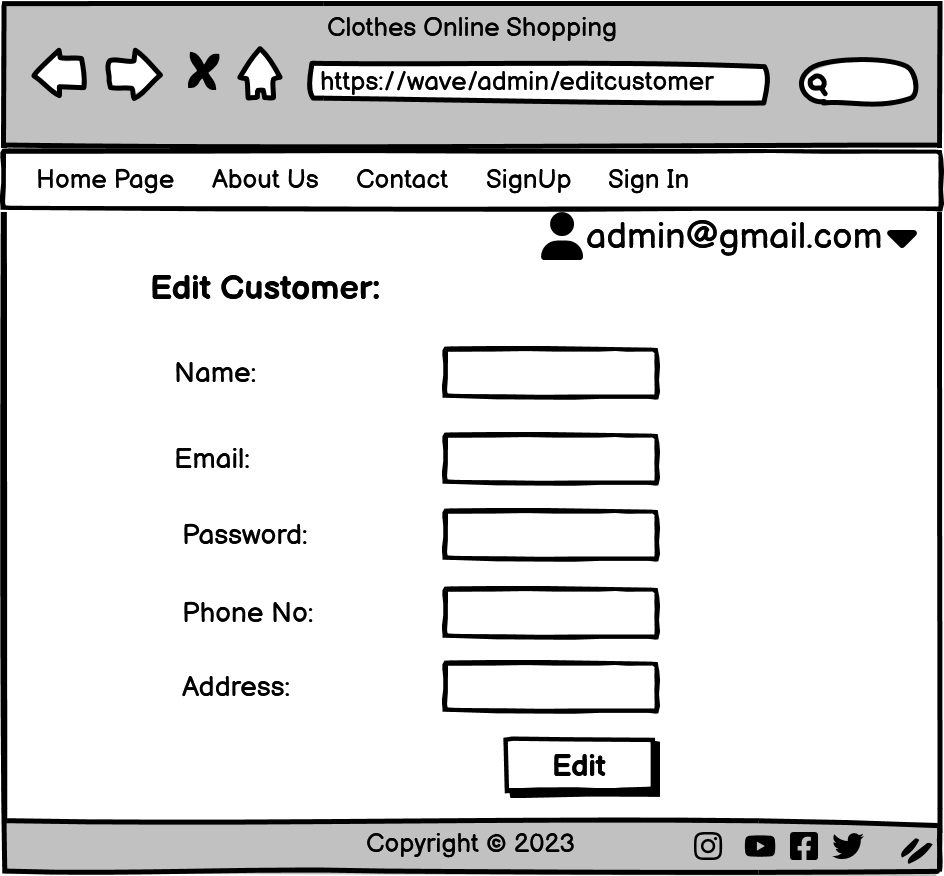
\includegraphics[scale=1.]{images/Edit Customer.png}}
\caption{Edit Customer Page}
\label{fig}
\end{figure}

\newpage
\subsection{Product Details Page}
\bigskip
\paragraph{}
In Product Details page, there is a table that contains all the products' detailed information like product ID, description, categories, qty, etc. Website admins can see and modify the products information, add new product or delete an existing one. Select one product from the table and then click Edit button, admins can edit that product's information. Or by clicking the Delete button, admin can delete one existing product from website and also from the database. On the other hand, if admin want to add new product to the system, he/she click the Add button and add product.
\bigskip
\bigskip
\bigskip
\begin{figure}[h]
\centerline{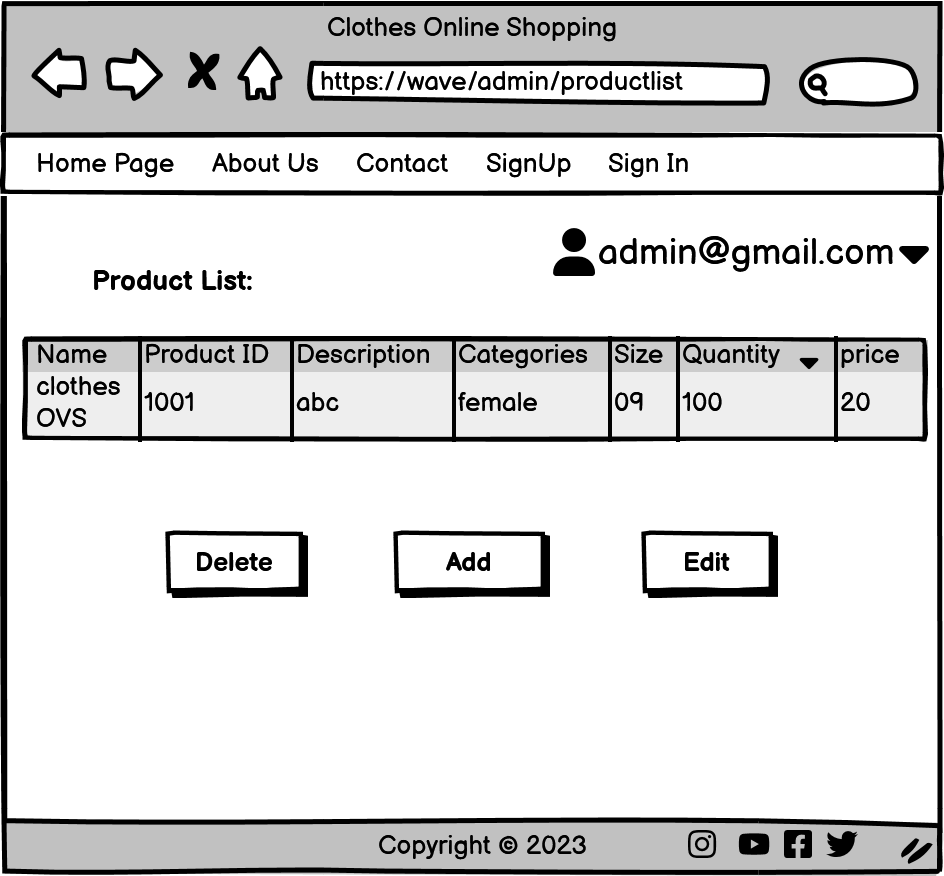
\includegraphics[scale=1.]{images/Product Details.png}}
\caption{Product Details Page}
\label{fig}
\end{figure}

\newpage
\subsection{Add Product Page}
\bigskip
\paragraph{}
In Add Product page, admin will fill manually the required fields; product ID, product name, price, quantity, size, description, etc and also image(s) of that product. Then, click the Add button at the end of the page. By clicking the Add button, new product is created and added to the system and database. Customers can add this new product to their cart. 

\bigskip
\bigskip
\bigskip
\begin{figure}[h]
\centerline{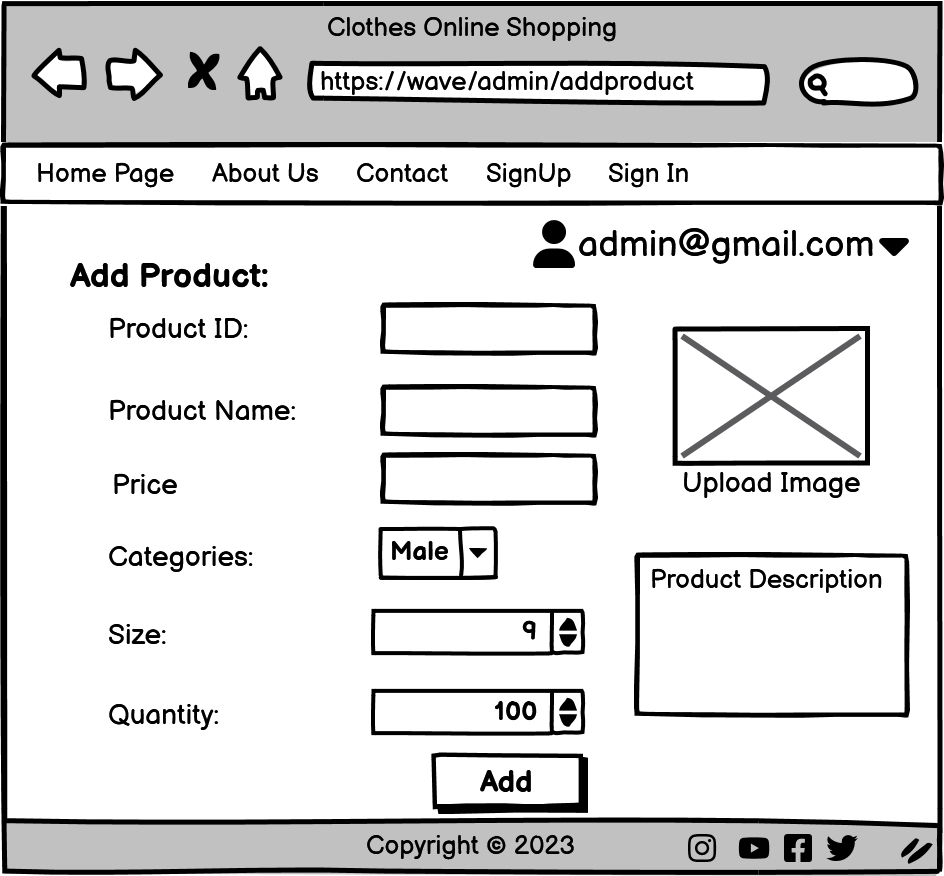
\includegraphics[scale=1.]{images/Add Product.png}}
\caption{Add Product Page}
\label{fig}
\end{figure}

\newpage
\subsection{Edit Product Page}
\bigskip
\paragraph{}
In Edit Product page, admins can see a product's information in details and change them. After changing the fields, they click the Edit button and submit the changes to the database. 
\bigskip
\bigskip
\bigskip
\begin{figure}[h]
\centerline{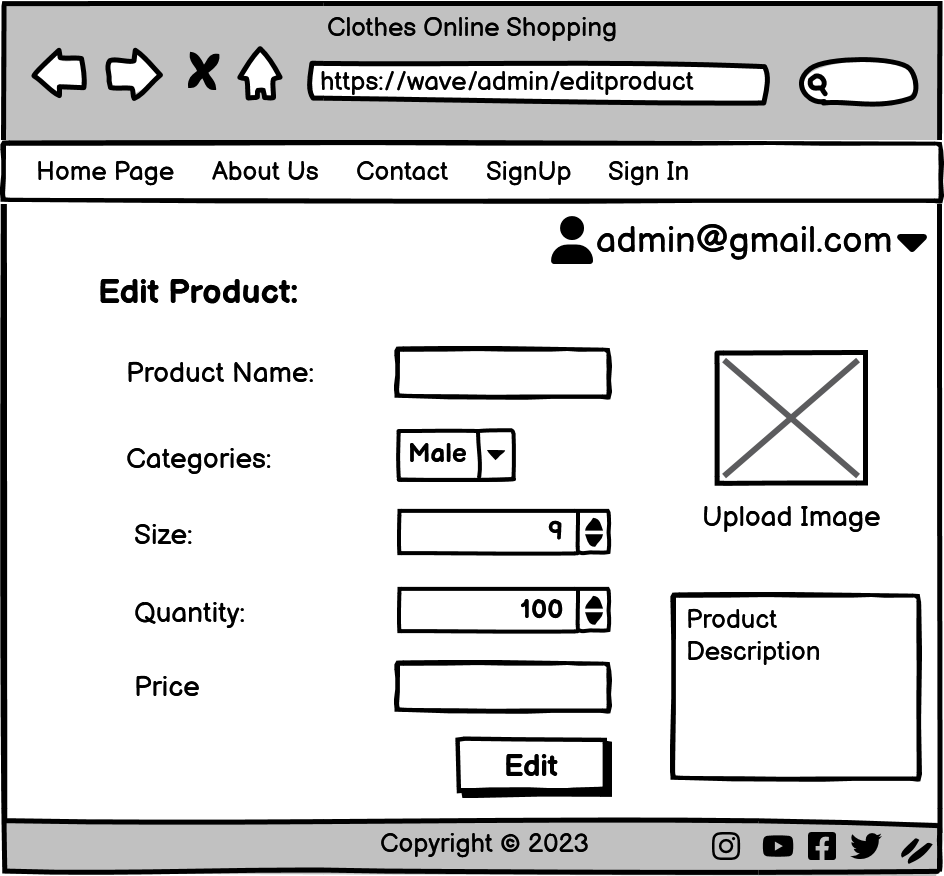
\includegraphics[scale=1.]{images/Edit Product.png}}
\caption{Edit Product Page}
\label{fig}
\end{figure}

\newpage
\subsection{Cart Page}
\bigskip
\paragraph{}
In Cart page, customers can see the products they choose to add in cart with details. In this page, they can change the product's amount, increase or decrease it or remove the product from the cart for good. After finalizing the shopping, customers can click the ... button and go to the next section which is giving the order.
\bigskip
\bigskip
\bigskip
\begin{figure}[h]
\centerline{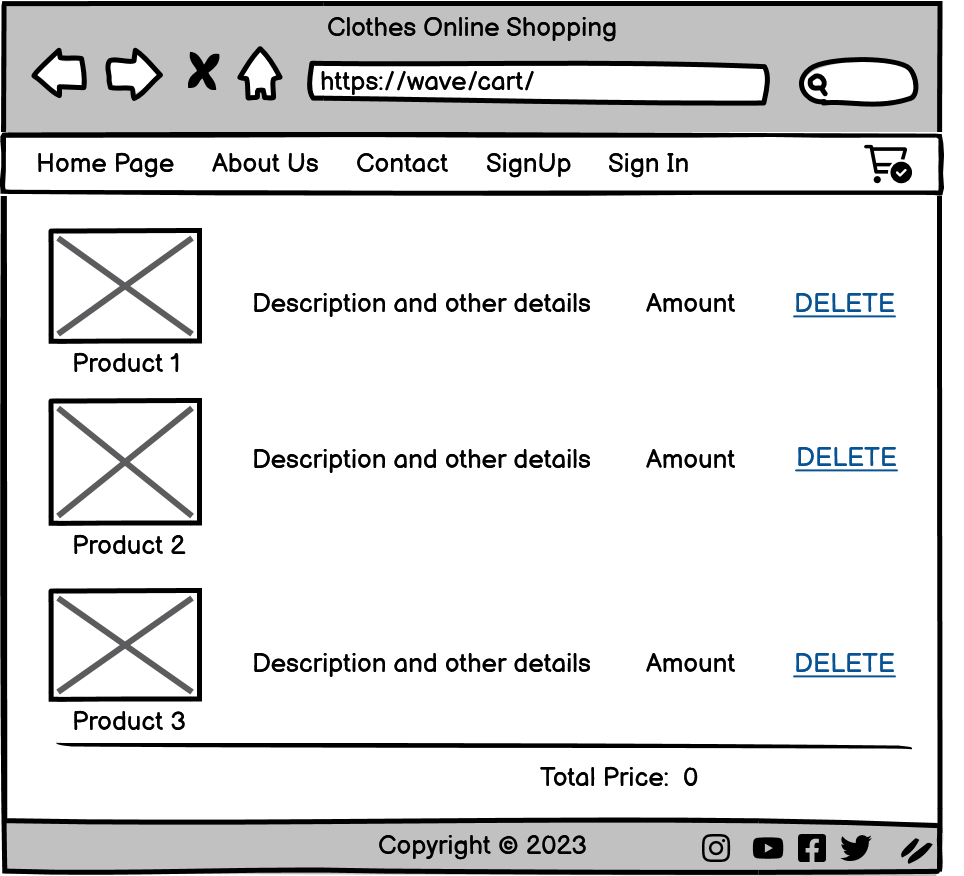
\includegraphics[scale=1.]{images/Cart.png}}
\caption{Cart Page}
\label{fig}
\end{figure}


\newpage
\section{Business Logic Layer}
\bigskip
\paragraph{} 








\end{document}